\documentclass{beamer}
\usetheme{Rochester}
\usepackage{amsmath}
\usepackage{graphicx}
\begin{document}
\title{The Exponential and Gamma Distributions}
\author{Arthur Lui and Alexis Cottam}
\date{October 9, 2013}

\def\wl{\par \vspace{\baselineskip}}

\begin{frame}
\titlepage
\end{frame}

\begin{frame}{The Exponential Distribution}
\[
  f(x \vert \beta) = \frac{1}{\beta}e^{(-x/\beta)}, 0 \leq x < \infty, \beta > 0
\] 
The parameter $\beta$ is a scale parameter.
\begin{center}
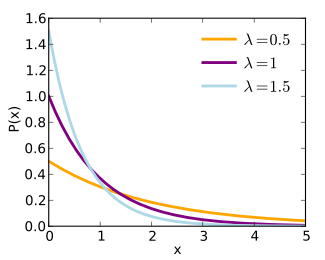
\includegraphics[scale=.50]{exppdf.png}
\end{center}
Note: $\lambda = \frac{1}{\beta}$
\end{frame}

\begin{frame}{CDF}
\[
  F(x) = 1 - e^{(-x/\beta)} , 0 \leq x < \infty
\]
\begin{center}
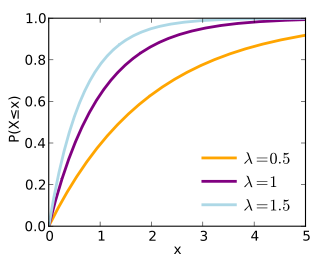
\includegraphics[scale=.50]{expcdf.png}
\end{center}
Note: $\lambda = \frac{1}{\beta}$

\end{frame}


\begin{frame}{Exponential Mean, Variance, and MGF}
\[
E(X) = \beta
\]
\[
Var(X) = \beta^2
\]
\[
M_{x}(t) = \frac{1}{1-\beta t} , t<\frac{1}{\beta}
\]
\end{frame}

\begin{frame}{Relationship to Other Distributions}
The Exponential Distribution is related to the Uniform, Gamma and Weibull Distributions.\\
\wl
If $X\sim Uniform$ and $Y=-log(X)$, then $Y\sim Exp$.\\
If $X\sim Gamma(\alpha = 1, \beta)$, then $X\sim Exp(\beta)$.\\
If $X\sim Exp$ and $Y=X^{(1/\gamma)}$, then $Y\sim Weibull$.\\
\wl
The Exponential Distribution is the continuous form of the Geometric Distribution.
\end{frame}

\begin{frame}{Example of Exponential Distribution}
If the average waiting time at a doctor's office is $\beta = 20$ minutes, what is the probability that you will have to wait less than 10 minutes?
\[
P(X \leq 10) = \int_0^{10} f(x)\mathrm{d}x = 0.3934693
\]
\end{frame}

\begin{frame}{More about the Exponential Distribution}
The exponential distribution can also be used to model time between Poisson events and lifetimes.\\
\wl
An interesting characteristic is that the Exponential distribution is memoryless.
\[
P( X > s | X> t) = P(X > s-t)
\]
For example: Given you have waited 20 minutes, the probability you'll wait 30 minutes is the same as the probability you'll wait 10 minutes.
\end{frame}

%%%%%%%%%%%%%%%%%%%%%%%%%%%%%%%%%%%%%%%%%%%%%%%%%%%%%%%%%%%%%%%%%%%%%%%%%
\begin{frame}{Gamma Function:}
    The Gamma Function is defined as:
    \[
      \Gamma (\alpha) = \int\limits_0^\infty {t^{\alpha - 1} e^{-t} dt},
    \]
    where $\alpha > 0$.
\end{frame}

\begin{frame}{Useful Identities:}
    Properties of the Gamma Function:
    \[
      \Gamma(\alpha+1) = \alpha\Gamma(\alpha), ~~~\alpha > 0
    \]
    \[
      \Gamma(n) = (n-1)!, ~~~ n ~ \epsilon ~ \mathbb{N}
    \]
    \[
      \Gamma(1) = 1
    \]
    \[
      \Gamma(\frac{1}{2}) = \sqrt{\pi}
    \]
\end{frame}

\begin{frame}{Gamma Distribution:}
  If $X \sim Gamma(\alpha,\beta)$, then the pdf of X is:
  \[
    f(x) = \frac{1}{\Gamma(\alpha)\beta^\alpha}  x ^ {\alpha-1}  e^{-x/\beta} 
  \]
  \begin{center}
  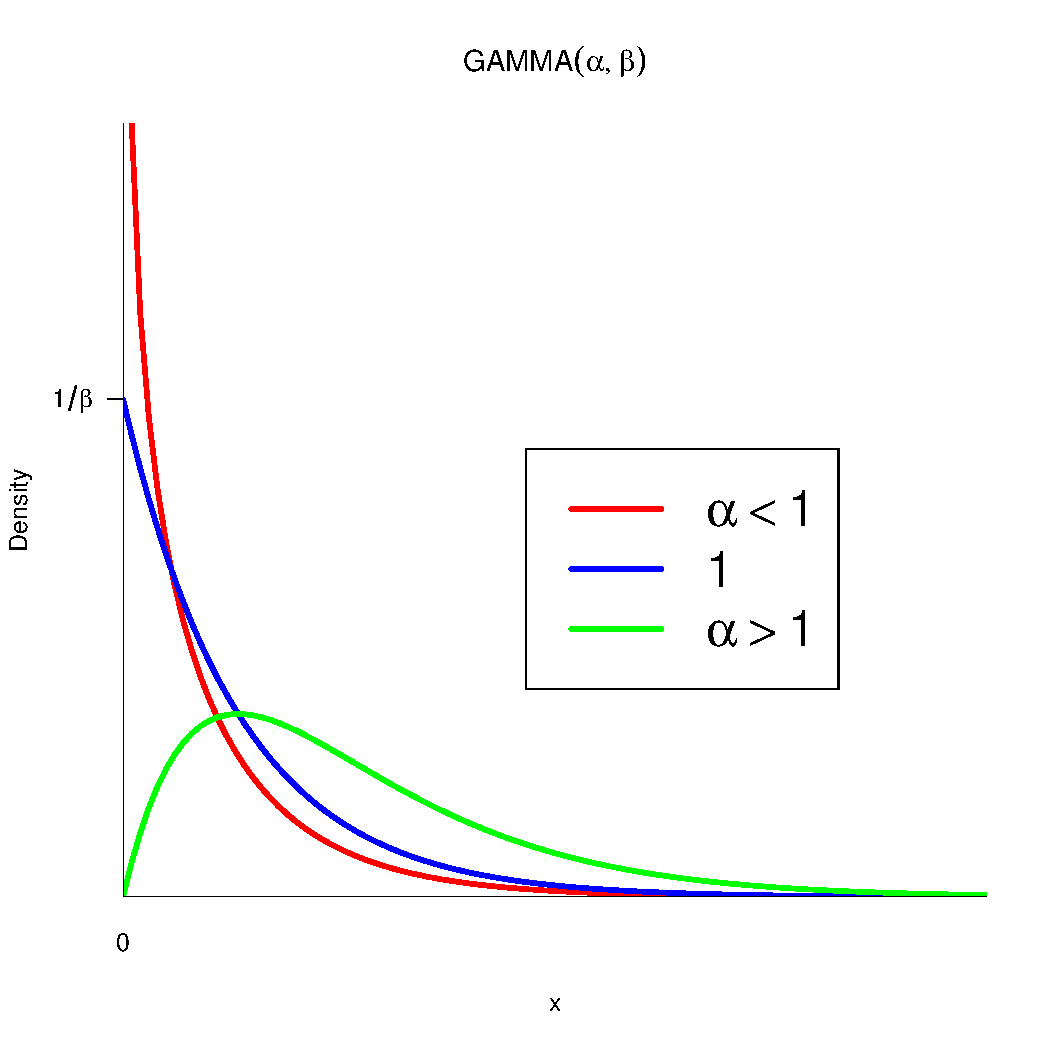
\includegraphics[scale=.3]{plot.pdf}
  \end{center}
\end{frame}
\begin{frame}{Gamma Distribution:}
  And the CDF is:
  \[
    \frac{\gamma(k,x/\theta)}{\Gamma(k)},
  \]
  where $k > 0$, and
  \[ 
    \gamma(k,x/\theta) = \int\limits_0^{x/\theta} {t^{k-1}e^{-t}dt}
  \]
\end{frame}

\begin{frame}{Gamma Mean, Variance, and  Moment Generating Function:}
Mean:
\[
  E[X] = \alpha \beta
\]
Variance:
\[
  Var[X] = \alpha  \beta ^ 2 
\]
MGF:
\[
  M_x(t) = \left( {\frac{1}{1-\beta t}} \right) ^ \alpha
\]

\end{frame}

\begin{frame}{Relation to Other Distributions:}
  \textbf{Poisson-Gamma.} The Gamma distribution is a conjugate prior 
  for the mean of the Poisson distribution.\\
  \textbf{Exponential-Inverse Gamma.} The Inverse Gamma distribution is a 
  conjugate prior for the mean of the exponential distribution. \\
  \wl
  \textbf{Exponential.} $Gamma(1,\beta) = EXP(\beta)$.\\
  \textbf{Chi-Sqaured.} $Gamma(p/2,2) = \chi ^2 (p)$.\\
  \textbf{Maxwell.} Let X be distributed as a Gamma. If $\alpha = 3/2$, then $Y = \sqrt{X/\beta}$ is distributed as a Maxwell.\\
  \textbf{Inverse Gamma.} Let $X \sim Gamma(\alpha,\beta)$. Then $Y = 1/X \sim InverseGamma(\alpha,\beta)$.\\
\end{frame}

\begin{frame}{Relation to Other Distributions:}
  \textbf{More on Poisson-Gamma.} The Negative Binomial can be derived as a gamma mixture of Poissons.\\
  \wl
  Specifically, if
  \[
     X \sim NB (r,\beta)
  \]
  and
  \[
    X|\lambda \sim POI(\lambda),
  \]
  then
  \[
    \lambda \sim Gamma(r,\beta).
  \]
\end{frame}

\begin{frame}{Applications of the Gamma Distribution:}
  The Gamma distribution is positive and right-skewed, so it is can be used to model a variety of events, including the following:\\
    \wl 
    - The amount of rainfall accumulated in a reservoir\\
    - The size of loan defaults of aggregate insurance claims\\
    - The flow of items through manufacturing and distribution processes\\
    - The load on web servers\\
    - The many and varied forms of telecom exchange
\end{frame}

\begin{frame}{Very Hypothetical Situation:}
  Suppose that for a graduate Statistical Computing course, the average time required for every student to come up with a feasible solution for each exam problem is two hours. Compute the probability that a student, say Mickey, will take 8 or more hours to come up with the solutions to all four problems of the exam.\\
\wl
One problem every 2 hours means we would expect to "solve" $\beta = 1/2$ exam problems every hour on average. Using $\beta = 1/2 $ and $\alpha = 16$, we can compute this as follows:
\[
  P(X \ge 8) = \int\limits_8^\infty {\frac{x^{16-1}e^{-x/.5}}{\Gamma(4)2^{16} }dx}
             = .466745
\]

Hypothetical Inference???
\end{frame}

\end{document}
